%-------------------------------------------------------------------------------
%-------------------------------------------------------------------------------
%-------------------------------------------------------------------------------
\chapter{Sudoku}
%-------------------------------------------------------------------------------
%-------------------------------------------------------------------------------
\thispagestyle{empty}
%-------------------------------------------------------------------------------
%-------------------------------------------------------------------------------
%-------------------------------------------------------------------------------
{\it Le jeu de Sudoku se joue sur une grille 9x9.

On remplit les cases par des chiffres entre 1 et 9 de telle sorte que chaque ligne, chaque colonne et chacun des 9 carrés 3x3 contienne les 9 chiffres.

\begin{center}
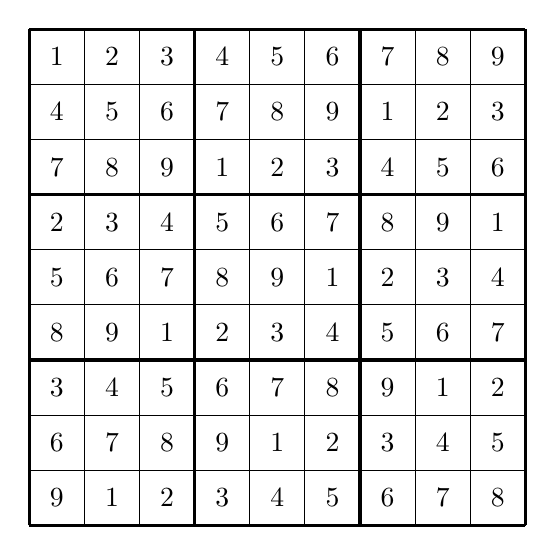
\begin{tikzpicture}[scale=0.7]
\tikzstyle{every node}=[draw,minimum size =7mm,fill=white]
\foreach \n [count=\i from 0] in {1,4,7,2,5,8,3,6,9}
{\foreach \j  in {0,1,2,3,4,5,6,7,8}
\pgfmathtruncatemacro\k{mod(\j +\n-1,9)+1}
 \node[rectangle]  (l\i\j) at (\j,{9-\i}) {\k};}
\foreach\i in {0,3,6,9}
 {\draw[very thick] (-0.5,{\i+0.5}) -- (8.5,{\i+0.5});
 \draw[very thick] ({\i-0.5},0.5) -- ({\i-0.5},9.5);}
\end{tikzpicture}
\end{center}
}
%-------------------------------------------------------------------------------
%-------------------------------------------------------------------------------
%-------------------------------------------------------------------------------
\section{Définition} 
%-------------------------------------------------------------------------------
%-------------------------------------------------------------------------------
%-------------------------------------------------------------------------------
Nous allons utiliser un constructeur somme pour les cases :
%-------------------------------------------------------------------------------
\begin{lstlisting}
type contenu = Vide | Pleine of int ;;
\end{lstlisting} 
%-------------------------------------------------------------------------------
On pourra représenter les grilles par des tableaux de tableaux, on nommera \type{sudoku} ce type.
%-------------------------------------------------------------------------------
%-------------------------------------------------------------------------------
\begin{Exercise}
{\'Ecrire une fonction qui crée une grille vide. Sa signature sera  \type{init : unit -> sudoku}
}
\end{Exercise}
%-------------------------------------------------------------------------------
\begin{Answer}
\begin{lstlisting}
let init () =
  Array.make_matrix 9 9 Vide;;
\end{lstlisting} 
\end{Answer}
%-------------------------------------------------------------------------------
%-------------------------------------------------------------------------------
\begin{Exercise}
{\'Ecrire une fonction qui copie une grille dans une grille indépendante.
}
\end{Exercise}
%-------------------------------------------------------------------------------
%-------------------------------------------------------------------------------
\begin{Answer}
\begin{lstlisting}
let copie grille =
  let g = init() in
  for i = 0 to 8 do
    for j = 0 to 8 do
      g.(i).(j) <- grille.(i).(j) done; done;
  g;;
\end{lstlisting} 
\end{Answer}
%-------------------------------------------------------------------------------
%-------------------------------------------------------------------------------
\begin{Exercise}Créer la grille présentée au début.
\end{Exercise}
%-------------------------------------------------------------------------------
\begin{Answer}
\begin{lstlisting}
let exemple =
  let g = init() in
  let un = [|1; 4; 7; 2; 5; 8; 3; 6; 9|] in
  for i = 0 to 8 do
    for j = 0 to 8 do
      g.(i).(j) <- Val ((un.(i)+j-1) mod 9 + 1) done; done;
  g;;
\end{lstlisting} 
\end{Answer}
%-------------------------------------------------------------------------------
%-------------------------------------------------------------------------------
\begin{Exercise}\'Ecrire une fonction \type{imprime : sudoku -> unit} qui imprime une grille.
\end{Exercise}
\begin{center}
\begin{lstlisting}
 --- --- ---
|5xx|xxx|xxx|
|xxx|x7x|xxx|
|xx8|xxx|xxx|
 --- --- ---
|xxx|xxx|xxx|
|xxx|xxx|xxx|
|xxx|xxx|xxx|
 --- --- ---
|xxx|xxx|xxx|
|xxx|xxx|xxx|
|xxx|xxx|xxx|
 --- --- ---
\end{lstlisting} 
\end{center}
%-------------------------------------------------------------------------------
\begin{Answer}
\begin{lstlisting}
let imprime grille =
  let h = " --- --- ---\n" in
  print_newline ();
  print_string h;
  for i = 0 to 8 do    
    print_string "|";
    for j = 0 to 8 do
      (match grille.(i).(j) with
       |Vide -> print_string "x"
       |Val(n) -> print_int n);
      if (j+1) mod 3 = 0
      then print_string "|" done;
    print_newline ();
    if (i+1) mod 3 = 0
    then print_string h done;;
\end{lstlisting} 
\end{Answer}
%-------------------------------------------------------------------------------
%-------------------------------------------------------------------------------
%-------------------------------------------------------------------------------
\section{Jouer}
%-------------------------------------------------------------------------------
%-------------------------------------------------------------------------------
%-------------------------------------------------------------------------------
%-------------------------------------------------------------------------------
\begin{Exercise}\'Ecrire une fonction \type{possible grille i j n} qui renvoie un booléen indiquant s'il est licite de placer la valeur $n$ à la ligne $i$ et la colonne $j$ de la grille. On devra vérifier les 3 conditions.
\end{Exercise}
%-------------------------------------------------------------------------------
\begin{Answer}
\begin{lstlisting}
let verif grille lg col n =
  let rep = ref true in
  for i = 0 to 8 do
    if i <> lg && (case grille i col) = Val(n)
    then rep := false;
    if i <> col && (case grille lg i) = Val(n)
    then rep := false done;
  let a = lg/3 and b = col/3 in
  for i = 0 to 2 do
    let u = 3*a + i in
    for j = 0 to 2 do 
      let v  = 3*b +j in
        if (u <> lg || v <> col) && (case grille u v) = Val(n)
        then rep := false done; done;
  !rep;;
\end{lstlisting} 
\end{Answer}
%-------------------------------------------------------------------------------
%-------------------------------------------------------------------------------
\`A présent nous allons résoudre des grilles avec contraintes, c'est-à-dire partiellement remplies. Pour cela on utilisera une méthode assez naïve qui va essayer toutes les solutions possible jusqu'à en trouver une bonne. On appelle cette méthode ''backtracking'' car on revient en arrière quand on tombe sur un cul-de-sac.
%-------------------------------------------------------------------------------
\begin{itemize}
\item On tente d'insérer un 1 dans la première case vide.
%-------------------------------------------------------------------------------
\item Si c'est possible alors on passe à la case suivante
%-------------------------------------------------------------------------------
\item Quand on aboutit à une impossibilité on passe à 2 puis 3 \dots
%-------------------------------------------------------------------------------
\item Si on arrive à 9 sans trouver de solution, on retourne à la case précédente pour y essayer le nombre suivant
\end{itemize}
%-------------------------------------------------------------------------------
%-------------------------------------------------------------------------------
\begin{Exercise}\'Ecrire la résolution d'une grille.
\end{Exercise}
%-------------------------------------------------------------------------------
\begin{Answer}
\begin{lstlisting}
exception Solution;;

let suivant (i,j) =
  if j = 8
  then (i + 1,0)
  else (i,j + 1);;

let resoudre grille = 
  let g = copie grille in
  let rec aux g (lg,col) = 
    if lg = 9
    then raise Solution
    else if case g lg col <> Vide
         then aux g (suivant (lg,col))
         else for n = 1 to 9 do
                if possible g lg col n
                then (g.(lg).(col) <- Val n;
                      aux g (suivant (lg,col));
                      g.(lg).(col) <- Vide) done in
  try aux g (0,0);
      failwith "pas de solution"
  with Solution -> imprime g;;
\end{lstlisting} 
\end{Answer}
%-------------------------------------------------------------------------------
%-------------------------------------------------------------------------------
On pourra utiliser une exception pour arrêter dès qu'on a trouvé une solution.
%-------------------------------------------------------------------------------
\begin{lstlisting}
exception Solution;;

let resoudre grille =
  ...
  let aux ...
    ...
    if ... 
    then raise Solution
    ...
  try aux ...
      ...
  with Solution -> imprime g;;
\end{lstlisting} 
%-------------------------------------------------------------------------------
%-------------------------------------------------------------------------------
%-------------------------------------------------------------------------------
\section{Aller plus loin}
%-------------------------------------------------------------------------------
%-------------------------------------------------------------------------------
%-------------------------------------------------------------------------------
On peut compter le nombre de solutions

On peut alors construire des grilles qui n'ont qu'une solution.

\type{Random.int (n+1)}  renvoie un nombre au hasard entre 0 et n.
%--------------------------------------------------------------------------
%--------------------------------------------------------------------------
